\section{Theory} % 28-32 Seiten

	\subsection{Smart Home} 
		There is a necessity to provide a sweeping substantiated knowledge-base in order to develop smart home middleware. Hence basic terms like \textit{home} have to be defined which later build up the basis for justification on decision taking in the development process.

		\subsubsection{What is a home?}
			The general definition of a home \textit{the place where a person (or family) lives \parencite{websters1}} is not sufficient enough for the domain of smarter home. Due to this fact information on the term \textit{home} is collected and used to create a suitable definition. The famous citation of Louis Sullivan \textit{form follows function} further used as \textit{Sullivans rule}, originally altered from papers of nature observation where Horatio Greenough came to the conclusion that form only changes if function changes \parencite{FFF} also applies to buildings such as homes. The following figure shows a plan of a house where every room has its specific functions assigned to it:

			\pagebreak

			\begin{figure}[h]
				\centering
					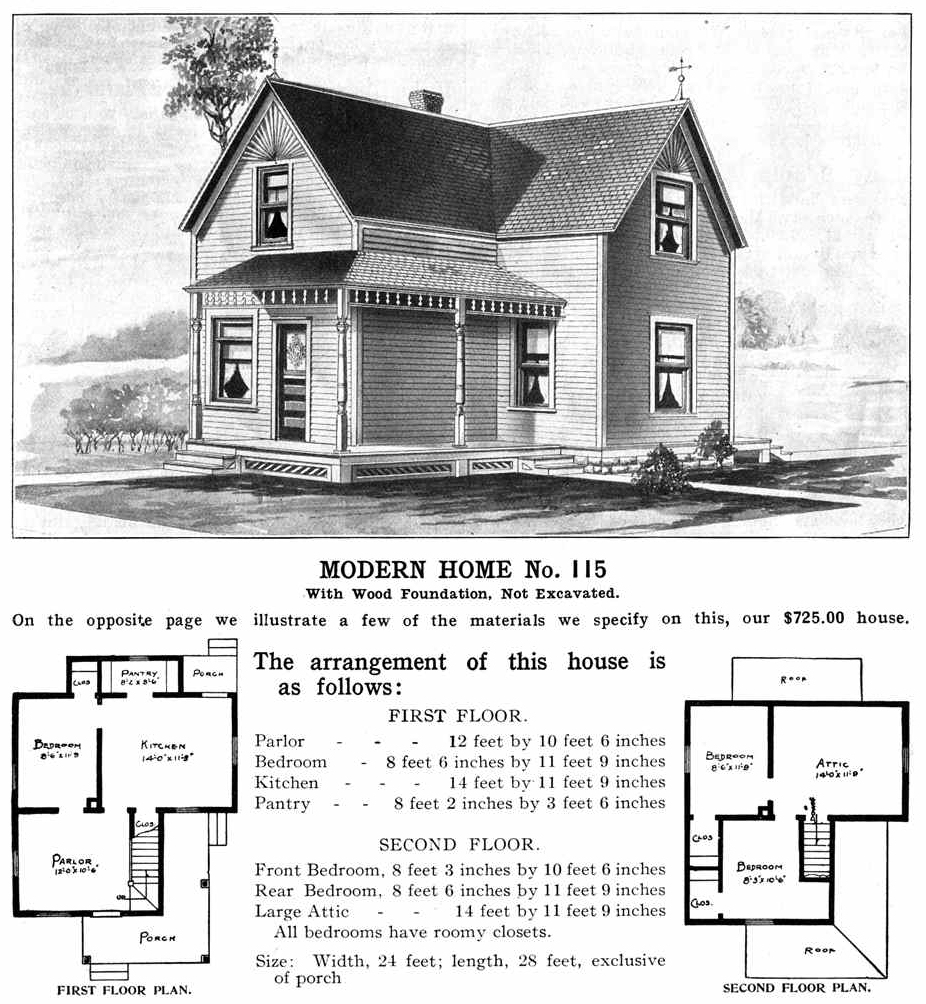
\includegraphics[width=.9\textwidth]{images/theory/RoomFunctions.jpg}
				\caption{Social functions for rooms}
				\label{fig:RoomFunctions}
			\end{figure}

			\pagebreak

			Since the function of a home is in general a place to live and the question of life is a little to complicated to clarify in this paper, more general abstractions are defined to meet the daily approaches on living. The National Institute of Schooling started an approach on naming the functions of a home \parencite{homeFunctionality}:

			\begin{itemize}
				\item Protective
				\item Economic
				\item Religious
				\item Educative
				\item Social
				\item Affectional
				\item Status-giving
			\end{itemize}

			These functions are the root for further more complex and current \textit{daily needs} which are not discussed further due too unnecessary specific information. Religious, Educative, Affectional and Status-Giving functions are not considered as necessary for a good smart home implementation and therefore not applied later. Further a home is a geographical location like a city or suburb and used as a permanent or semi-permanent residence, whereas transitory accommodations (hospital, prison, college, etc) are not considered as home but in the scope of smart home.\\

			%\subsubsection{\textit{Definition: Home}}

			%\subsubsection{\textit{Definition: House}}

		\subsubsection{Smart home use cases}\label{posInCS}
		Smart Home use cases are pretty much bound to the services that are run. So in the following table some services are provided as use cases:

		\begin{table}[h]
			\centering
			\caption{Homekit Accessory Profiles}
			\label{Homekit_Accessory_Profile}
			\begin{tabular}{ll}
				\textbf{Services}		& \textbf{Characteristics} \\
				\hline
				Garage door openers		& Lock state \\
				Lights					& Brightness \\
				Door Locks				& Lock state \\
				Thermostats				& Current temperature \\
				IP camera controls		& Model number \\
				Switches				& Switch state \\
				Custom					& Custom
			\end{tabular}
		\end{table}

		These services represent actions that can be performed with the help of smart home devices. A more general way of describing use cases for smart home is done by naming the functions it has to serve in order to accomplish the given actions.\\ 

		\subsubsection{Definitions: Smart home - iot}
			To get an inside view smart home and suitable iot definitions are shown below:

			\begin{itemize}
				\item \textbf{Smart home} “Smart Home is the topic for technical procedures inside of houseings that are supposed to improve indoor environment and living quality, security and efficient energy using remotely controlled devices.” \textcite{}

				\item \textbf{IoT} “the Internet of Things (IoT) refers to identifiable objects and their virtual representation in an Internet-like structure.” \parencite{IoTDef1}

				\item \textbf{IoT} “moving small packets of data to a large set of nodes, so as to integrate and automate everything from home appliances to entire factories.” \parencite{IoTDef2}

				\item \textbf{IoT} “the term commonly is used to signify advanced connectivity devices, systems and services that go beyond machine-to-machine communications, and covers a variety of protocols, domains and applications.” \parencite{IoT-Techcrunch}
			\end{itemize}

			\textbf{Smart home, general things to keep in mind}
				The following list is an aggregation of the previous definitions:

				\begin{itemize}
					\item improvement of indoor environment and living quality
					\item improvement of security
					\item improvement of energy efficiency
					\item devices are remotely controlled
					\item devices are identifiable objects and have a virtual representation
					\item actions are automated
				\end{itemize}

		\subsubsection{\textit{Feature-ism}}
			Computing power hasn't increased much since 2010, a more stagnating trend is visible. Companies like Intel are improving power consumption instead of computing power because there is a physical end, namely the size of transistors can't get any smaller. The idea is to scale in width rather than height, which means more cores instead of more power \parencite{CPUComputingPower}. So we have come to the point that the everyday user is used to the fact that computing power won't increase drastically anymore \parencite{CPUComputingPower}. To keep the users buying and attracted to new hardware tricks have to be played. Samsung and many others know the path of feature-ism to keep the users attracted to their devices. Every year all new features that "revolutionize" the user experience are thrown into the market and cause technological entanglement \parencite{TechnologicalMinimalism}. New feature are always "cool" to show them to your friends, but longterm thoughts suffer. Users are "often enticed by the lure of interesting and exotic technologies that look like fun, but in the end, they don't serve us very well for what we want to achieve."\parencite{TechnologicalMinimalism} John Martellario, a writer for the MacObserver mag, states that: "there is only a proper, considered subset of all the available technologies out there that are required to get any specific job done." \parencite{TechnologicalMinimalism} With that idea in mind and combined with the Sullivans rule minimalism in technology is what makes it useful and good. Later on measurements are also taken on future proof ness because its aim able and necessary to create a worthwhile user experience \parencite{TechnologicalMinimalism}. 

		\subsubsection{Mapping of smart home and basic home functions}
			There is little information about valuation methods for IT systems in the internet that cover topics like usability for the user and extensibility as well as futer proof ness, instead dozens of financial valuing methods. Due to this fact the definitions of smart home are aggregated and mapped to the basic functions of a home in order to provide use cases for a proper valuation.

			\begin{table}[h]
				\centering
				\caption{Mapping of smart home services to basic home functions}
				\label{Homekit_Accessory_Profile}
				\begin{tabular}{ll}
					\textbf{Smart home}	& \textbf{home functions} \\
					\hline
					Indoor environments			& Economic and Social \\
					Living quality				& Social \\
					Security					& Protective \\
					Energy efficiency			& Economic \\
					Remotely controlled			& Protective and Economic \\
					Identifyable devices 		& Protective and Economic \\
					Automation					& Protective and Economic \\

				\end{tabular}
			\end{table}


			\subsubsection{Final measurements}

				These smart home functions have to be mappable to basic home functions. Due to the fact that device functions do not change when replaced by smart home devices, the amount of set up and carry on work should be as low as possible: \textit{minimalism}. Moreover \textit{Where function does not change, form does not change \parencite{SullivansRule}}, implies that the absence of minimalism namely extra hardware is negatively valued. A switch is still a switch and shouldn't need to be connected to extra hardware in order to work. smart home devices are costly and therefore should be future proof and not fall into the garbage whenever a new version hits the market. \\

				For economic reasons costs of requiered hardware, installation and maintenance have to be considered. Due to the fact that IBM doesn't provide homegateway hardware, costs have to be roughly evaluated from current systems on the market not considering the purchase price. %Overall costs are mapped to two different categories. First a family with two children, secondly a single household and later on given by costs per person. In the case of the family the costs are distributed to the parents without charging the kids.
				\\
				The following list shows all measurements that are considered in this thesis:

				\begin{itemize}
					\item security
					\item smart home functions
						\begin{enumerate}
							\item feature-ism 
						\end{enumerate}
					\item cross compatibility
						\begin{enumerate}
							\item sullivans rule / minimalism
							\item futureproofness
						\end{enumerate}
					\item costs
					\item other
				\end{itemize}

				%\begin{figure}[h]
				%	\centering
				%		\includegraphics[width=1\textwidth]{images/theory/SmartHomeMeasurements.png}
				%	\caption{Overview of Smart Home measurements}
				%	\label{fig:SmartHomeLandscape}
				%\end{figure}

				Further the evaluation is done on values ranging between +2 for excellent fullfillment all to -1 for not fullfilling the requirements.

				\begin{figure}[h]
					\centering
						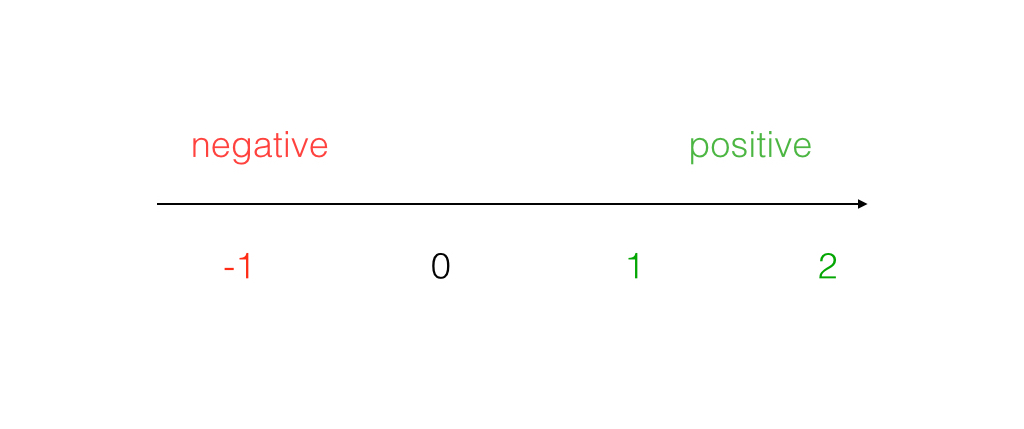
\includegraphics[width=.9\textwidth]{images/praxis/Evaluation.jpg}
					\caption{Evaluation Overview}
					\label{fig:SmartHomeLandscape}
				\end{figure}
		
				\pagebreak

	%########################################################################
	%BASIC APPROACHES FOR SMART HOME
	%########################################################################
	\subsection{Current Systems}
		In the scope of this thesis more familiar and emerging smart home solutions in the sheer flood of vendors are discussed. Therfore the selection of vendors for a basic analysis are the following:

		\subsubsection{Apple HomeKit} 
			\textbf{Overview}
				Apple builds up its functionality on two radio systems: WiFi and Bluetooth Low Energy. Where all HomeKit enabled devices connect directly to an iDevice there is also a possibility of connecting a HomeBridge which serves more radio and cable systems in order to connect more decent devices. Since version 2.0 Homekit comes with the possibility of using the Apple TV as a tunnel to the internet. All iDevices that are registered to the same Apple ID can communicate to each other for a home automation interaction. Further approaches do not rely any more on the Apple TV. Third party HomeBridges are enabled to take communication over the internet. The iCloud itself will serves as a switchboard where iDevices can communicate to all HomeKit enabled ones. Currently there are no news on a car connection or further approaches into smart cars.

				\begin{figure}[h]
					\centering
						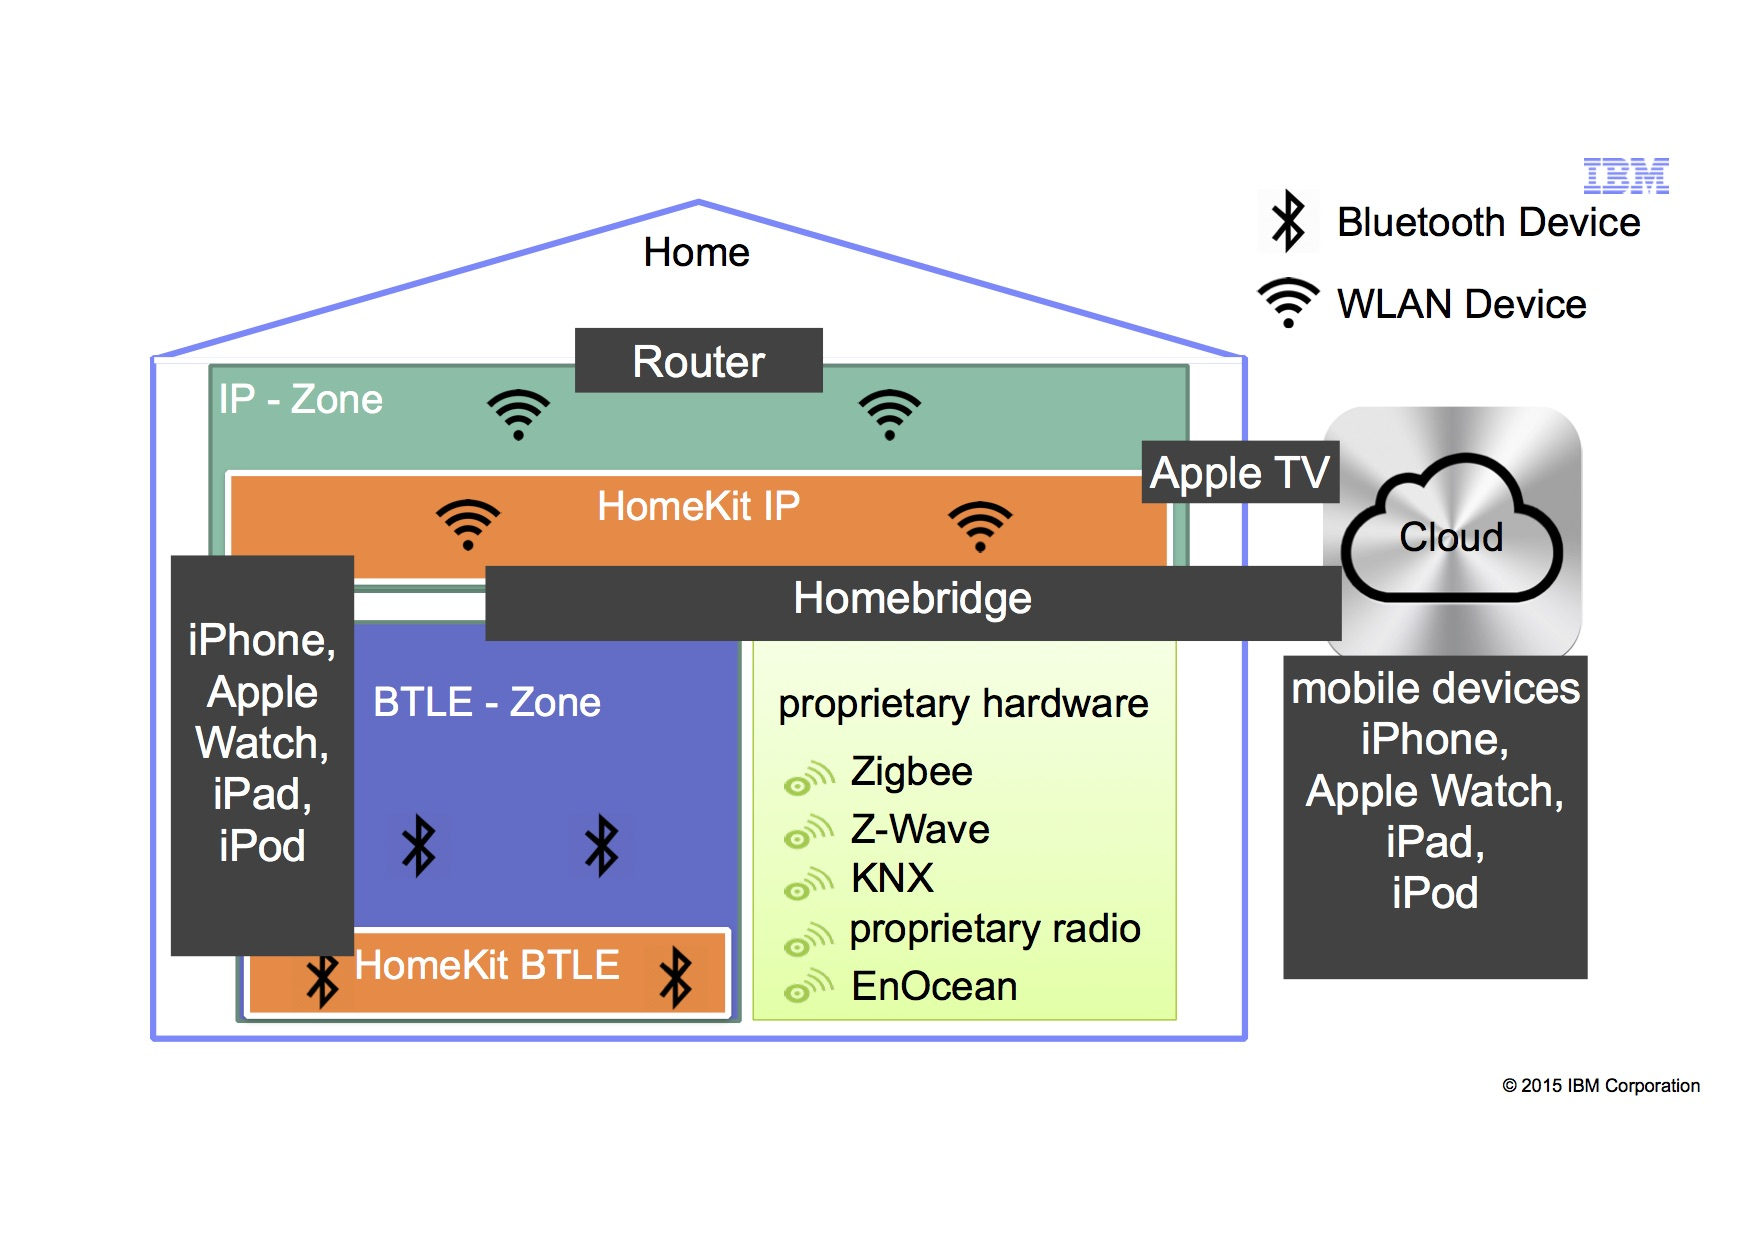
\includegraphics[width=.9\textwidth]{images/theory/SmartHomeLandscape.jpg}
					\caption{Overview of Apple HomeKit functionality}
					\label{fig:SmartHomeLandscape}
				\end{figure}

				\pagebreak
 
		\subsubsection{Samsung Smart Home}
			\textbf{Overview}
				Samsung Smart Home solution provides connectivity between all connected devices at home with a single app that can be accessed from smart phones, tablets, tvs and watches. Further information about Samsungs Smart Home solution is rare but three key features are explained below:\\

			\textbf{Device Control}
				Device Control allows the user to interact with several home devices. Moreover voice control is implemented and enables the possibility to use special phrases like "I am leaving" to trigger predefined action sets like turning of the lights, the air condition and start the cleaning robots \parencite{SHP}.\\

			\textbf{Smart Customer Service}
				The Smart Customer Service notifies the user whenever a smart device needs to be cleaned or repaired \parencite{SHP}.\\

			\textbf{Home View}
				Home View is considered as a sort of home surveillance system featuring connected cameras to monitor everything happening at home \parencite{SHP}.\\

			It should be mentioned that at the current state only devices out of Samsungs own product line are supported for smart home purposes. Nevertheless Samsung claims third party support witch the aid of its Smart Home Protocol \parencite{SHP}.

			%\pagebreak

		\subsubsection{SmartThings}
			\textbf{Overview}
				SmartThings started as a Kickstarter project and was acquired by Samsung in 2014. The idea behind it is a combination of a hub and an app. The hub provides the interconnect ability to other devices and aggregates communication for the app. In other words the app can talk to devices from multiple vendors. This is made possible by supporting additional radios compared to HomeKit and Samsung Smart Home namely Zigbee and Z-wave. A big downside is the absence of voice control. Only with more or less elaborate workarounds it is possible to control your devices with your voice \parencite{SmartThingsKick}.

				\pagebreak

		\subsubsection{Google Smart Home}
			\textbf{Overview}
				In 2014 Google acquired the Smart Home specialist Nest with its productline consisting of a thermostat (Nest Thermostat) and a smoke sensor (Nest Protect) \parencite{GoogleAcquiresNest}. After nearly one and a half year of silence in Googels smart home sector Nest revealed the Nest Cam, a 1080p smart home connected camera. For additional \$ 10 per month the user acquires the ability to review video material of the last 10 days as well as getting notifications from nest whenever suspicious activity is detected.\\

			\textbf{Brillo}
				"Brillo extends the Android platform to all your connected devices, so they are easy to set up and work seamlessly with each other and your smartphone"\parencite{Brillo}. With Brillo comes Weave which serves a consistent api for device communication. An instant communicaiton with Android is guaranteed by the developers at Google \parencite{BrilloHeise}. The bedrock of Brillo is a downscaled version of Android supposed to run on systems with low hardware specks like smart home devices \parencite{BrilloHeise}.

				\pagebreak



	%########################################################################

	%########################################################################
	\subsection{Battle for Standards}

		\subsubsection{Home gateway solution}
			Insteon, Lutron and many others competing in the HomeKit market aren't developing dedicated devices to connect to Apples Smart Home solution. The common answer is a bridge which serves as an allocator for connecting existing smart home devices. Where Elgato is the pioneer with it's EVE series on dedicated devices.\\

		\subsubsection{Radios}
			Where the market in the industry is ruled by radio systems like Zigbee and Z-wave, the smart home segment is more common radio systems friendly by using widely spread technology like WiFi and Bluetooth Low Energy.\\

		\subsubsection{Cross compatibility}	
			It doesn't matter how good every single solution on smart home is on it self. For many users the usage and the installation of multiple vendors solutions is difficult. So cross compatibility is desirable. Approaches on this topic are poorly solved with bridges that are able to connect more devices to an existing platform than it actually supports.\\

		\subsubsection{Fog underneath the cloud}
			These bridges have to have more logic components than end devices in order to pre filter information and handle communication over different radios. An in official term for that kind of technology is the fog. The fog itself stands for logical pre computation before pushing information to the cloud.\\

		\subsubsection{Market dominance}
			The market dominance is at the moment not important because there is no standard in smart home communication. When thinking back to the early ages of the internet a top dog like http and ip where only possible by defining standards. And rash decisions on the market leader are not appropriate in terms of iot.\\

		\subsubsection{User VS company}
			It remains the question if the user drives the development of new smart home technology or the companies do.\\

			\pagebreak


	%########################################################################

	%########################################################################

	\subsection{Technologies}

			\subsubsection{HomeKit enabled}
				\textbf{Lutron Electronics}
					, a company born when electricity was rare and lightbulbs were generating that much heat that they were rather used to boil some eggs than to read a book at night. It's founder Joel Spira was a pioneer in dimmable lights, a technology former only known in theatre. Spira liked the idea of saving energy and money by dimming lights. 1959 he filled out his first patent of a dimmable switch which would fit into a wall plug, revolutionary at that time. Nowadays Lutron holds over 2,700 worldwide patents, one of them is a window shading technology \parencite{lutron}. In 2015 Lutron steps into the HomeKit smart home area by revealing a new bridge which can be controlled over an iOS app as well as Siri and Apple Watch. All existing caseta and caseta wireless devices can be connected to the bridge.\\

				\textbf{Insteon Technologies}
					Insteon Technologies is a home automation company which was founded by Joe Dada in 1992 and has coined the term smart home. In January 2015 Insteon announced a gateway (bridge) to allow an interconnection with the Apple HomeKit system.\\

				\textbf{Elgato Eve}
					Elgato started with Eve it's HomeKit compatibility, where all devices are equipped with Bluetooth Low Energy to connect directly to an iDevice like the iPhone.\\

			\subsubsection{Non-HomeKit}
				\textbf{Raspberry Pi}
					There are multiple HomeKit accessory bridge implementations for the Raspberry Pi including HAP-Java.
					%, which relies on the reverse engineering work of Alex Skalozub.\\

				\textbf{Belkin WeMo}
					Belkin WeMo is a series of lights, switches and sensors that come with a dedicated app. Control takes place over WiFi where nearly every device is able to connect itself to the local network.\\

			\subsubsection{Radios}
				Belkin is more the home approach for an automation where Zigbee and Z-wave are more top dogs in the industry.

				\textbf{Zigbee}
					Zigbee is a specification for low powered radio devices which are used for small data rates, perfect for home automation.\\ 

				\textbf{Z-wave}
					Z-wave itself is pretty close to Zigbee.\\

				\pagebreak

	%########################################################################

	%########################################################################
	\subsection{HomeKit and SDPvNext}

		\subsubsection{Apple HomeKit}

			\textbf{Apple HomeKit} is an API developed by Apple. A common database stores all home information to provide consistency and is available to all Apps. Users can use Siri to interact with their home accessories. Homekit also provides remote access and uses end to end encryption between iDevices in order to maintain user privacy and security \parencite{IntroToHomeKit}. 

			\begin{figure}[h]
				\centering
					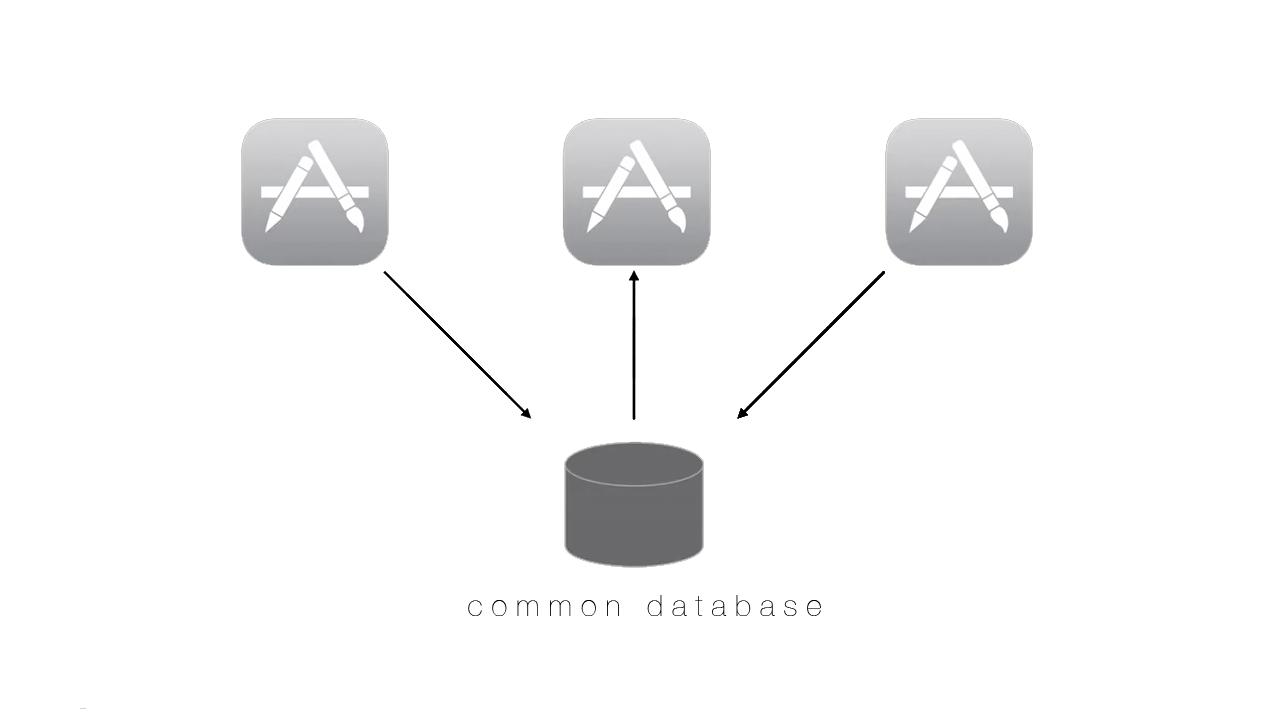
\includegraphics[width=.9\textwidth]{images/theory/Homekit_Database.png}
				\caption{Common database provided by HomeKit \parencite{IntroToHomeKit}}
				\label{fig:Homekit_Database}
			\end{figure}

			\textbf{The Home Manager} is the entry point for all apps. With the help of the Home Manager changes to the database are made. Homes can be added or removed and will notify the user in case of changes \parencite{IntroToHomeKit}.

			The organigram used by Homekit is build up by \textbf{Homes}. Homes create their own namespace and have to be named uniquely, contain Rooms and Accessories. Rooms have to be named uniquely in their Home domain. \parencite{IntroToHomeKit}\\

			\textbf{An Accessory} corresponds to a physical device and is assigned to a Room. Accessory Objects allow to access the device state \parencite{IntroToHomeKit}.\\

			\textbf{Services} represent functionality of an Accessory and are like parameters you can interact with. Services may have a name because some Services are not ment to interact with a user(update firmware). Services are a collection of \textbf{Characteristics} like range or units, e.g. the power state of a lightbulb Service. \parencite{IntroToHomeKit}.\\

			\textbf{Characteristics can be of a fiew variety:}

			\begin{itemize}
				\item read-only  - e.g. the current temperature 
				\item read-write - e.g. lightbulb power state
				\item write-only - e.g. identify accessorie
			\end{itemize}


			Homes, Rooms, Accessories, Services and Characteristics are recognized by Siri and can therefore be accessed without a direct interaction with an app, making the use of HomeKit very comfortable. Services have Apple defined types, that can be accessed by natural language like synonyms or expression that do not exactly refer to the correct name provided to the Service making interaction experience more natural like. \parencite{IntroToHomeKit}.\\

			\textbf{The Accessory Browser} is used to find any new Accessories available and is used to add them to a Home. When it is added to a Room it's time to name the Accessory and assign it to a Room \parencite{IntroToHomeKit}.\\

			\textbf{Initial setup workflow:} 

			\begin{itemize}
				\item Create a Home - User provides name
				\item Add Rooms to the Home - User provides names
				\item Add Accessories - Use an Accessory Browser - add Accessory to Home - User provides name - User chooses Room
				\item interact through application and/or Siri
			\end{itemize}

			A natural way of referring to Accessories in a Home is done by grouping. Apples HomeKit enables the user to group Accessories in several ways, name them and provide access to Siri \parencite{IntroToHomeKit}.:

			\textbf{Zones} are arbitrary, uniquely named groups of Rooms e.g. \textit{upstairs}, where Rooms can be in any number of Zones and are recognized by Siri \parencite{IntroToHomeKit}. 

			\begin{figure}[h]
				\centering
					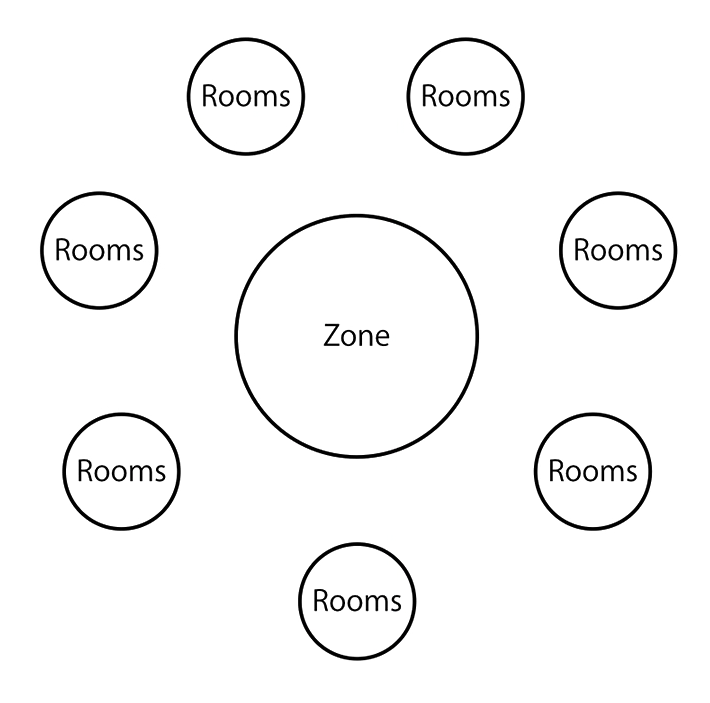
\includegraphics[width=.5\textwidth]{images/theory/Zones.png}
				\caption{Zones \parencite{IntroToHomeKit}}
				\label{fig:Homekit_Database}
			\end{figure}

			\textbf{Service Groups}  are arbitrary, uniquely named groups of Services and are a convenient way to control Services across accessories e.g. \textit{nightlight} \parencite{IntroToHomeKit}.

			\begin{figure}[h]
				\centering
					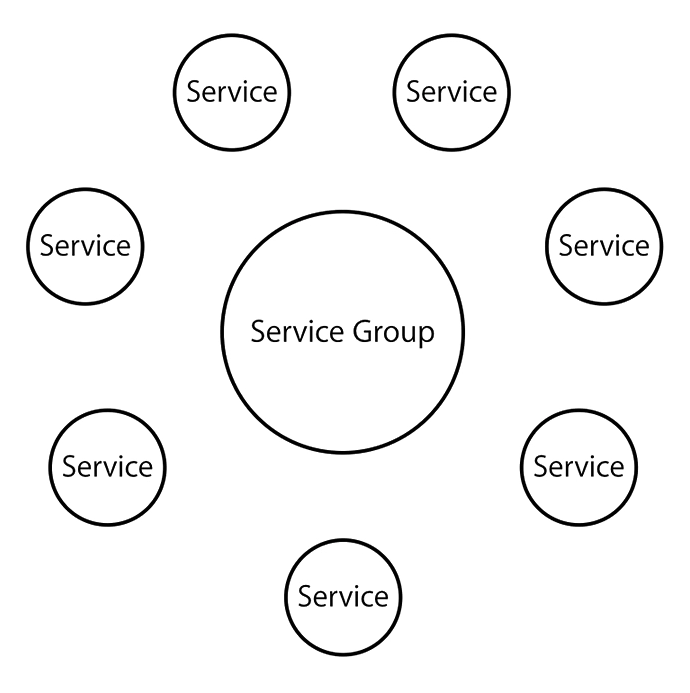
\includegraphics[width=.5\textwidth]{images/theory/Service_Groups.png}
				\caption{Service Groups \parencite{IntroToHomeKit}}
				\label{fig:Homekit_Database}
			\end{figure}

			\textbf{Actionsets} Collection of actions that are executed together in an undefined order, e.g. \textit{night} \parencite{IntroToHomeKit}.

			\begin{figure}[h]
				\centering
					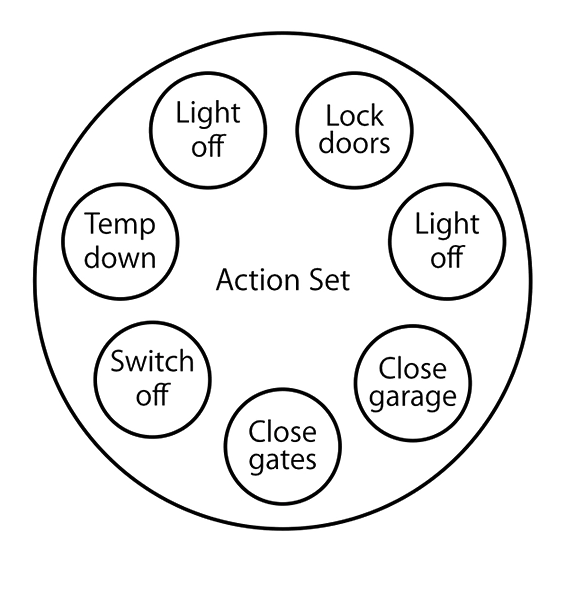
\includegraphics[width=.5\textwidth]{images/theory/Actionsets.png}
				\caption{Actionsets \parencite{IntroToHomeKit}}
				\label{fig:Homekit_Database}
			\end{figure}

			\pagebreak

		\subsubsection{WWDC15}

			\textbf{Security} All communication between the Accessories and Apple HomeKit are end to end encrypted. Moreover Keys for encryption are changed after each session. Keys are not able to decrypt data from the past or the future. All data is encrypted using keys that are local on the device which ensures privacy of data. Further on administrative features for user management are added.\\

			\textbf{Maintain existing objects} In order to guarantee uniqueness of Accessories, Apple has introduced a unique identifier (NSUUID) in iOS 9.\\

			\textbf{Predefind Scenes} are scenes that occur in a regular every day cycle. Apple has provided some standard scenes like:

			\begin{itemize}
				\item Get up
				\item Leave
				\item Return
				\item Go to bed
			\end{itemize}

			Moreover these predefined scenes can not be deleted but customized and are recognized by Siri. These scenes are managed action sets, as known from iOS 8. Visual clues are information that are added by an Accessory Category.

			\textbf{Apple Watch} Homekit is now available on watchOS2. All the home data is mirrored on the Apple Watch. Homes can be viewed, Accessories can be controlled and scenes can be executed by hand or over Siri.\\

			\textbf{Event Triggers} Scenes that are executed at specified times of the day are known from iOS8. Events respond to the state of an Accessory or location based events by using geofences. Furthermore Events can be triggered:

			\begin{itemize}
				\item Time-based
				\item Significant events like:
					\begin{itemize}
						\item Surise
						\item Sunset
					\end{itemize}
			\end{itemize}

			Time based triggers can be used in a natural way. One way to use them is to specify a time-based trigger to fire after 6pm another to trigger on Sundays. Every trigger can be used in logical addition. To tie it all together every trigger has an associated scene which will be executed when the trigger is fired.\\

			\textbf{Remote Access} allows the user to control their Accessories even if they are not at home. In order to get access to that feature the user needs an Apple TV 3rd gen. Verification is done by using the same Apple ID on both devices. For users without an Apple TV remote access is managed with the \textit{Homekit Accessory Protocol (HAP)} over iCloud. This means that you can control your Accessories and get notifications without an Apple TV, no matter where you are.\\ 

			\textbf{Bluetooth Low Energy} The distance to an Accessory is crucial in order to control it over BTLE. Devices that are to far away from the user cannot be controlled. A secure connection is possible in iOS9 by HAP secure tunneling provided by an intermediate device. The Accessory is connected over BTLE to the intermediate device which is then exposed as an Object over WiFi. The range extender will also be able to provide remote access to all connected BTLE Accessories that works with HomeKit. To ensure privacy the intermediate device can not see the content of the HAP protocol.\\

			\textbf{Notifications} BTLE Accessories fully support notifications and metadata for custom characteristics. Notifications transported over different channels are recognized by the iDevice featuring iOS9 as redundant.\\

			\textbf{Programmable Switches} are used to map this event to a trigger and execute a scene. This feature is very powerful and useful to map an amount of actions to physical switches.\\

		\subsubsection{HAP - HomeKit Accessory Protocol}

			\textbf{Transports} There are two ways to connect Accessories to HomeKit, one is BTLE the other one is over IP.\\

			\textbf{Security} is achieved by \textit{Bi-directional authentication} and \textit{Per-session} encryption.\\ 

			\textbf{Bi-directional authentication} or mutual authentication is a technology where both parties involved in authentication are aware of each other. This means that the server is authenticating itself to the user as well as the user is authenticating itself to the server. The term \textit{Authentication} describes the process of confirming identities and is done by verifying the validity of a client with a digital certificate.\\

			\textbf{SSL} is a "cryptographic protocol designed to provide communication security over a computer network". The way that SSL works is by "authenticating the counterpart with whom they are communicating and to negotiate a symmetric key". "This session key is then used to encrypt data flowing between the parties". "An important property in this context is forward secrecy, so the short-term session key cannot be derived from the long-term asymmetric secret key". SSL is initialized in layer 5 (Session Layer) of the ISO/OSI model and has a handshake using an asymmetric cipher in order to establish cipher settings and shared key for that session. Afterwards the presentation layer (ISO/OSI 6) is providing the encryption fo the data.\\

			\textbf{Network}\\ 

		\subsubsection{Siri}
			HomeKit itself is an app independent service running in the background like Siri. Siri is Apples own natural language interpreter which is able to answer questions and perform actions on spoken and written user commands. Actions can be delegated to third party web services like Wolfram Alpha or in the domain of this thesis actions can control smart devices. Apple has logically concatenated the HomeKit database with Siri to enable seamless interaction between both services.\\

		\subsubsection{iDevices}

			\textbf{Apple TV}
				The Apple TV serves as a tunnel to the outside world in order to access your smart home devices from everywhere internet is accessible.\\

			\textbf{iPhone}
				The proprietary HomeKit service is running in the background of all iDevices and can be accessed and managed from all iDevices registered to the same Apple ID.\\ 

			\textbf{Apple Watch}
				The Apple Watch serves as an external display for iPhones. Further more it is packed with a microphone as well as a speaker which makes the watch perfect for interacting with Siri and your home.\\

		\subsubsection{Bluemix}
			Bluemix is an upcoming web service of IBM based on OpenStack software where users can create environments to test their code. Several programming languages are supported among them Java and NodeJS. Further there is a possibility to host an IoT environment called IoT Foundation. This service is backed up with a database and able to connect to IoT Foundation clients of your choice. The clients are devices which are able to connect them selves to the internet and build up an connection to the IoT Foundation - smart home devices. Because of the fact that the devices have to handle ip communication its standing to a reason that they mostly serve as home gateways which are connected to more proprietary smart home devices.\\

		\subsubsection{IoT Foundation}
			The IoT Foundation is the smart home cloud solution of IBM where configured gateways connect themselves over mqtt to the cloud.\\ 

			\begin{figure}[h]
				\centering
					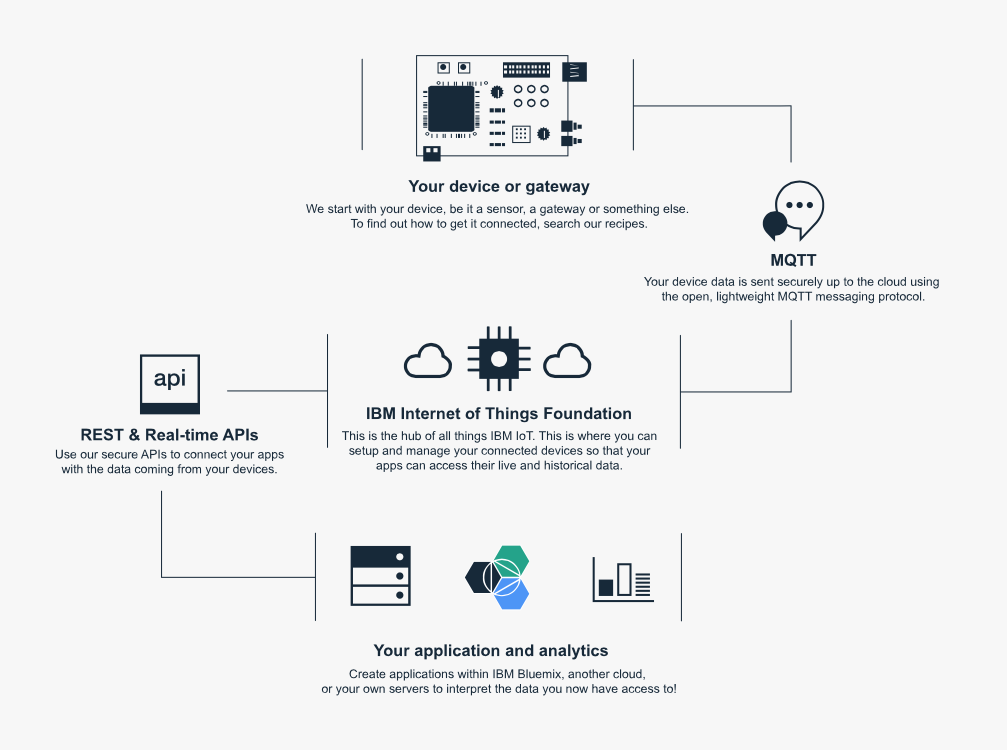
\includegraphics[width=.9\textwidth]{images/theory/IoTFoundationOverview.png}
				\caption{IoT Foundation overview \parencite{IoTFoundationOverview}}
				\label{fig:SmartHomeLandscape}
			\end{figure} 

			\textbf{Organizations}
				IBM implemented the model of organizations into their home automation solution. After registration on the Internet of Things Foundation website a unique organization ID consisting of a  six character identifier is paired to your account. Data from devices and applications are only accessible with the organization ID. Applications are bound to the organization ID by so called API keys. Once an Application connects itself to the IoT Foundation it is directly bound to the organization ID which owns the Api key. Cross-organization communication is not implemented due to security reasons \parencite{IoTFoundationOverview}.\\

			\textbf{Devices}
				A device is per IBMs definition anything that can connect itself to the internet "and has data it wants to get into the cloud" \parencite{IoTFoundationOverview}. Further a devices is not able to interact with other devices, however it accepts commands from applications. Devices can only be managed when registered to the IoT Foundation with a unique authentication token \parencite{IoTFoundationOverview}.\\

			\textbf{Applications}
				An Application is like a device anything that has a connection to the internet, but interacts with multiple devices. Applications have to identify them as well as devices. Additionally to the authentication token an application has to register itself to the IoT Foundation with an Api key \parencite{IoTFoundationOverview}.\\

			\textbf{Events}
				Data is published to the IoT Foundation with a mechanism called event, where devices control the content of an event as well as the name for each event \parencite{IoTFoundationOverview}. The IoT Foundation is performing identification checks with the help of credentials. Therefore every event can be mapped to a specific device. IBM even claims that "with this architecture it is impossible for a device to impersonate another device" \parencite{IoTFoundationOverview}. Further devices are unable to receive events, whether their own or from others. Applications are able to process events where they have access to the source of the event as well as the data it contains. "Applications can be configured to subscribe to all events from all devices, a subset of events, a subset of devices or a combination of these events" \parencite{IoTFoundationOverview}.\\

			\textbf{Commands}
				To accomplish communication between applications and devices a mechanism called \textbf{command} is used, where only applications can send commands to specific devices. On the other side actions performed after receiving commands on the device side have to be determined by the device itself.\\

			
		\subsubsection{SDPvNext Rest API}
			SDPvNext is the front end and user management system for the IoT Foundation service. Currently being integrated into the IoT Foundation and extending its functionality by adding an authentication layer to it. SDPvNext is equipped accessible by a Rest API which provides basic rest calls to get devices and their configurations.

			\pagebreak


	%########################################################################

	%########################################################################
	%\subsection{HAP-NodeJS}

		%\subsubsection{Node-Modules}

		%	\textbf{curve25519}

		%	\textbf{ed25519}

		%	\textbf{mdns}

		%	\textbf{node-persist}

		%	\textbf{srp}
	%########################################################################

	%########################################################################
	\subsection{Constraints}

		\textbf{HomeKit and SDPvNext}
			HomeKit and SDPvNext are the systems to connect in the course of this bachelor thesis.\\

		\textbf{HomeKit aatabase accessibility}
			The Homekit database is only accessible through iDevices, which means that only apps executed on an iPhone, iPad and iPod are able to add new devices to the HomeKit db.\\

		\textbf{SDPvNext Rest API}
			The given Rest API is limited to only read values in form of states out of the IoT Foundation. Thus restricting interaction with the platform to a unidirectional communication from SDPvNext to the iOS app. It is yet not stated whether adding or removing devices is possible through the rest API.\\

		%\textbf{Apple MFI}
			%Due to the fact that Apple is restraining their HAP-Protocol and it's functionality as well as every documentation on it to ensure just MFI certified developers are able to access it, it's nearly impossible to get any information on this topic. Hence this bachelor thesis relies on reverse engineered work from a Russian programmer Alex Skalozub.\\ 

		\textbf{General}
			This thesis is being written from June 1st until August 21st 2015. Apple itself released only rare information about the functionality of HomeKit on June 8th. Further more during this period there were no user or professional reviews on HomeKit devices since they just hit the market on 28 of July. Any experiences are gathered through simulation of devices and may not be equivalent or differ to real ones.\\

	%########################################################################

	%########################################################################
	\subsection{Development Tools} %this topic maybe better for praxis...

		\subsubsection{Mac OSX}

			\textbf{Xcode}
				Xcode is the standard tool to develop apps for iOS devices.\\

			\textbf{Hardware IO Tools for Xcode 6}
				In oder to test the functionality of apps being developed Apple makes a good job in device simulation. Due to the unavailability of real HomeKit devices the use of simulated ones is mandatory. Apple provides Hardware IO Tools to guarantee a testing environment which suits the real devices.\\

			\textbf{Homekit Accessory Simulator}
				The Homekit Accessory Simulator is used to simulate Accessories and Bridges and acts just like real accessories. By default every Accessory has an Access Information Service containing basic information like the name, manufacturer, model and serial number. Bridges are a special type of Accessory that provide the functionality of a Hub, whereas Hubs provide access to Accessories that can't connect themselves directly to iOS. Every Accessory provided by a bridge is listed as separate Accessory later in order to interact directly with it \parencite{IntroToHomeKit}.\\


	%########################################################################

	%########################################################################
	\subsection{Middleware}
		\textbf{Goal} The goal of this thesis is to develop a middleware which is capable of communicating with the IoT Foundation as well as the HomeKit database. Changes in either db's should be applied to the corresponding one by adding or removing devices from the databases (for additional information refer to constraints). Further the Apple Watch should be able to monitor and control the listed devices.

	\pagebreak
